\documentclass[12pt,oneside,a4paper]{article}
\usepackage{tabularx}
\usepackage{graphicx}
\usepackage[hidelinks]{hyperref}
\usepackage[top=1.2in]{geometry}
\usepackage{abstract}
\usepackage{setspace}
\usepackage{enumitem}
\usepackage[nodayofweek]{datetime}
\usepackage{cite}
\usepackage{times}
\usepackage{ragged2e}

\usepackage{lipsum}
\usepackage[table]{xcolor}
\usepackage{pdfpages}

\newcommand\todo[1]{\textcolor{blue}{#1}}
\newcommand\placeholder[1]{\todo{\lipsum[#1]}}

%%%%%%%%%%%%%%%%%%%%%%%%%%%%%%%%%%%%%%%%%%%%%%%%%%%%%%%%%%%%%%%%%%%%%%%

\definecolor{Green}{rgb}{0,0.7,0.1}

\providecommand\phantomsection{}

\tolerance=1
\emergencystretch=\maxdimen
\hyphenpenalty=10000
\hbadness=10000

\renewcommand{\abstractnamefont}{\normalfont\Large\bfseries}

\title{{\huge{IDENTIFY BLOOM KNOWLEDGE OF STUDENT}} \\ [30pt]
	\large{MINI PROJECT REPORT \\ SUBMITTED TO \\ [30pt] RAMAIAH INSTITUTE OF TECHNOLOGY} \\
	\normalsize{(Autonomous Institute, Affiliated to VTU)} \\ [10pt]
	\large{Bangalore - 560054} \\ [25pt]
	\normalsize\textsc{Submitted by} \\ [10pt]
	\begin{minipage}{0.6\textwidth}
		M Sneha \hfill 1MS14CS058 \\
		Mipsa Patel \hfill 1MS14CS148 \\
		Tilak S Naik \hfill 1MS14CS134 \\
		Vibha Karanth \hfill 1MS14CS136
	\end{minipage} \\ [30pt]
	\normalsize{As part of the Course \textbf{Data Analytics Laboratory - CSL717}} \\ [20pt]
	\large\textsc{SUPERVISED BY} \\
	\textbf{Parkavi. A} \\ \vfill
	
\includegraphics{rit.png} \\ [15pt]
	\large{DEPARTMENT OF COMPUTER SCIENCE \& ENGINEERING} \\ [5pt]
	RAMAIAH INSTITUTE OF TECHNOLOGY \\ [5pt]
	\large{Sep - Dec 2017}
	\thispagestyle{empty}
	\newpage
	Department of Computer Science and Engineering \\ [10pt]
	Ramaiah Institute of Technology \\
	\normalsize{(Autonomous Institute, Affiliated to VTU)} \\ [10pt]
	\large{Bangalore - 54} \\ [30pt]
	
\includegraphics{rit.png} \\ [20pt]
	\Large\textbf{CERTIFICATE} \\ [40pt]
	\normalsize \justify This is to certify that M Sneha (1MS14CS058), Mipsa Patel (1MS14CS148), Tilak S Naik (1MS14CS134), Vibha Karanth (1MS14CS136) have completed ``Identify Bloom Knowledge of Student'' as part of Mini Project. \\ [10pt]
We declare that the entire content embodied in this B.E. 7th Semester report contents are not copied. \\
	\vspace{\fill}
	\makebox[\textwidth]{
		\begin{minipage}{.4\textwidth}
			Submitted by \\ [10pt]
			M Sneha \hfill 1MS14CS058 \\
			Mipsa Patel \hfill 1MS14CS148 \\
			Tilak S Naik \hfill 1MS14CS134 \\
			Vibha Karanth \hfill 1MS14CS136 \\ [10pt]
			(Dept of CSE, RIT)
		\end{minipage}
		\hfill
		\begin{minipage}{.4\textwidth}
			\centering
			Guided by \\ [20pt]
			Prof. Parkavi \\
			Assistant Professor \\
			(Dept. of CSE, RIT)
		\end{minipage} \\
	}
	\thispagestyle{empty}
}

\author{}
\date{}

\begin{document}
	\maketitle
	\newpage
	\thispagestyle{empty}
	
	\centering
	Department of Computer Science and Engineering \\ [10pt]
	Ramaiah Institute of Technology \\
	\normalsize{(Autonomous Institute, Affiliated to VTU)} \\ [10pt]
	\large{Bangalore - 54} \\ [30pt]
	
\includegraphics{rit.png} \\ [10pt]
	\textbf{\underline{Evaluation Sheet}} \\ [20pt]
	\small
	\vspace{\fill}
	{\renewcommand{\arraystretch}{1.75}
		\begin{tabular}{|m{0.25cm}|>{\centering\arraybackslash}m{2cm}|>{\centering\arraybackslash}m{2.25cm}|>{\centering\arraybackslash}m{1.1cm}|>{\centering\arraybackslash}m{0.8cm}|>{\centering\arraybackslash}m{0.6cm}|>{\centering\arraybackslash}m{0.6cm}|>{\centering\arraybackslash}m{1cm}|>{\columncolor[HTML]{AAEDAC}}m{1cm}|}
			\hline
			 \textbf{Sl. No} & \textbf{USN} & \textbf{Name} & \textbf{Content and Demon-stration (15)} & \textbf{Speak-ing Skills (2)} & \textbf{Team work (2)} & \textbf{Neat-ness and care (2)} & \textbf{Effect-iveness \& Produc-tivity (4)} & \textbf{Total Marks (25)} \\
			\hline
			1 & 1MS14CS058 & M Sneha &&&&&&\\
			\hline
			2 & 1MS14CS148 & Mipsa Patel &&&&&&\\
			\hline
			3 & 1MS14CS134 & Tilak S Naik &&&&&&\\
			\hline
			4 & 1MS14CS136 & Vibha Karanth &&&&&&\\
			\hline
		\end{tabular}
	} \\
	\vspace{\fill}
	\normalsize
	\justifying
	Evaluated by \\ [10pt]
	\indent \indent
	\begin{minipage}{0.4\textwidth}
		Name: Parkavi. A \\
		Designation: Assistant Professor \\
		Department: Computer Science \& Engineering, RIT \\
		Signature:
	\end{minipage} \\
	\null \hfill HOD, CSE
	\newpage
	\thispagestyle{empty}
	\tableofcontents
	\newpage
	\pagenumbering{arabic}

	\null
	\vspace{\fill}

	\phantomsection
	\addcontentsline{toc}{section}{Abstract}
	\begin{abstract}
		\normalsize
		\doublespacing
		Each student has a different set of skills and strengths that they excel in. Their level of understanding in different concepts taught to them varies. It is important to identify their level of understanding, and one such metric to do so is Bloom’s Taxonomy of Learning Domains. Based on a student’s performance in questions belonging to different Bloom’s levels, he is classified into one of them. Identification of the cognitive domain of a student’s learning can help in improving his skills from one of the lower levels to higher levels that rely more on complex and abstract mental ability. 
	\end{abstract}

	\vspace{\fill}
	\null
	\newpage

	\section{Introduction}
		Bloom’s Taxonomy of Learning Domains identifies six levels within the cognitive domain, which are Knowledge, Comprehension, Application, Analysis, Synthesis and Evaluation. These domains range from the simple recall or recognition of facts, as the lowest level called knowledge, through increasingly more complex and abstract mental levels, to the highest order which is classified as evaluation. \\
		\\
		Given a set of questions that aim at evaluating the abilities of students in different learning domains, this project determines which level the students are best at. Two classifiers based on Naive Bayes and Support Vector Machines are used to classify the students’ marks into one of the levels, and the accuracy obtained using these models is compared. 



	\section{Literature Survey}

		\begin{description}[style=nextline]
			\item[\cite{ref:omar:2012} Automated analysis of exam questions according to bloom’s taxonomy - Nazlia Omara, Syahidah Sufi Harisa, Rosilah Hassana, Haslina Arshada, Masura Rahmata, Noor Faridatul Ainun Zainala \& Rozli Zulkiflib]
			This paper proposes an automated analysis of the exam questions to determine the appropriate category based on this taxonomy. This rule-based approach applies Natural Language Processing (NLP) techniques to identify important keywords and verbs, which may assist in the identification of the category of a question. \\

			\item[\cite{ref:lekha} Data Classification using Support Vector Machine - Durgesh K Srivastava, Lekha Bhambu]
			In this paper, a novel learning method, Support Vector Machine (SVM), is applied on different data (Diabetes data, Heart Data, Satellite Data and Shuttle data) which have two or multi class. SVM method does not suffer the limitations of data dimensionality and limited samples. It can be seen that the choice of kernel function and best value of parameters for particular kernel is critical for a given amount of data. \\

			\item[\cite{ref:awad:2004} An Effective Support Vector Machines (SVM) Performance Using Hierarchical Clustering - Mamoun Awad, Latifur Khan, and Farokh Bastani]
			This paper proposes a new approach for enhancing the training process of SVM when dealing with large data sets. It is based on the combination of SVM and clustering analysis. The idea is as follows: SVM computes the maximal margin separating data points; hence, only those patterns closest to the margin can affect the computations of that margin, while other points can be discarded without affecting the final result. \\

			\item[\cite{ref:lowd:2005} Naive Bayes Models for Probability Estimation - Daniel Lowd, Pedro Domingos]
			This paper proposes Naive Bayes models as an alternative to Bayesian networks for general probability estimation tasks. Experiments on a large number of datasets show that the two take similar time to learn and are similarly accurate, but Naive Bayes inference is orders of magnitude faster. \\
		\end{description}
		
		\section{Algorithm}
		
		\section{Implementation}
			The following 2 pages show an IPython Notebook that implements the algorithm.
			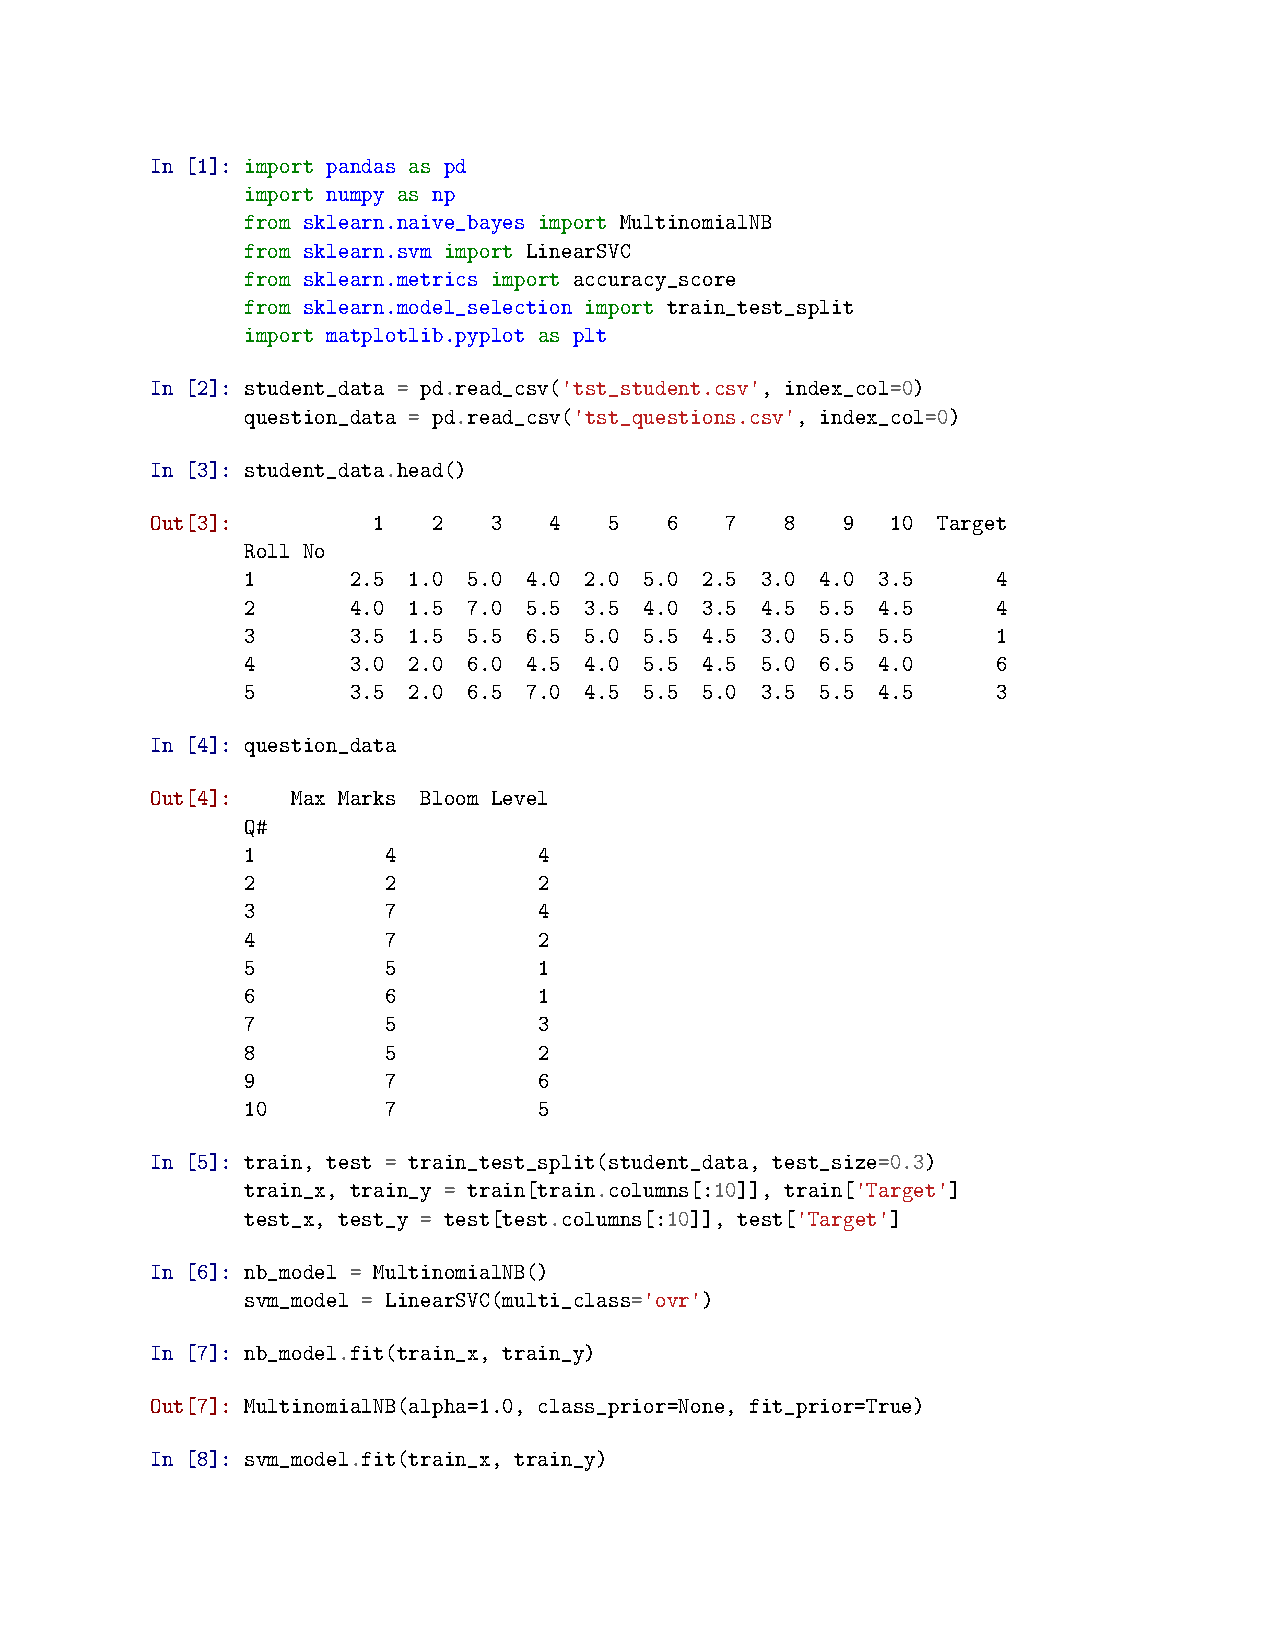
\includepdf[pages=-]{BloomLevelPredictor.pdf}
		
		\section{Results and Discussions}
		
		\begin{figure}
			\centering
			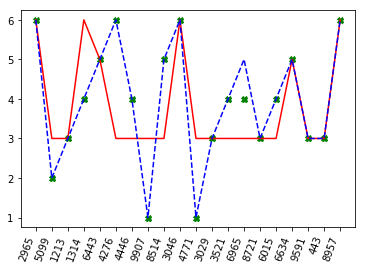
\includegraphics[scale=0.7]{BloomLevelPredictor.png}
			\caption{\small{The plot of Student ID vs Bloom Knowledge is shown. The green crosses indicate the actual target, the red solid lines indicate the predictions by Naive Bayes algorithm, and the blue dashed lines indicate the predictions by SVM.}}
			\label{fig:plot}
		\end{figure}
		
		Naive Bayes classifier gives an accuracy of $\approx 46\%$ without normalization, and $\approx 30\%$ with normalization. We observe that the accuracy of the Naive Bayes model does not increase significantly even on increasing the size of the dataset used to train the model.

		Comparatively, a model based on Support Vector Machines to obtain the Bloom’s level of a student gives an accuracy of $\approx 88\%$.
		
		A comparison for prediction on 20 student's data is shown in \autoref{fig:plot}.

		\section{Conclusion}
			Classification problems can be solved using various different approaches. In this project, we explore the use of two such algorithms. Naive Bayes algorithm gives a low accuracy in identification of bloom’s level. If we normalize before learning, the accuracy drops further. Support Vector Machine gives us a fairly good accuracy.

	\bibliographystyle{unsrt}
	\addcontentsline{toc}{section}{References}
	\bibliography{report}{}
\end{document}